\begin{figure}[!ht]
  \caption{ ~Virality of internet memes: \href{https://github.com/iworld1991/EpiExp/blob/master/Literature/bauckhage2011insights.pdf}{\cite{bauckhage2011insights}}}
  \label{fig:memes_curve}
    \subfloat[``salad fingers'']{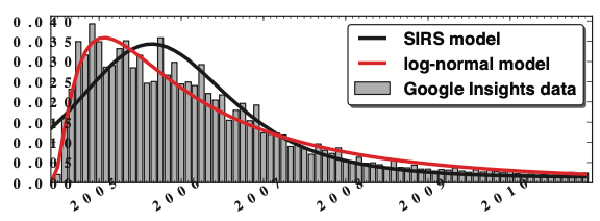
\includegraphics[width=\textwidth]{./figures/Memes1}}
    \newline
    \subfloat[``laughing baby'']{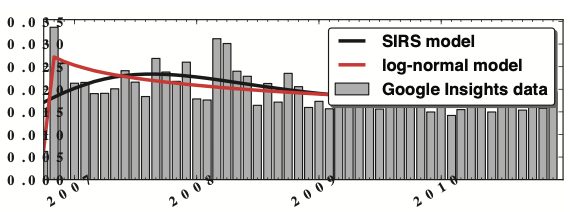
\includegraphics[width=\textwidth]{./figures/Memes2}}
    \newline
    \subfloat[``so much win'']{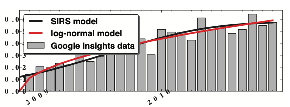
\includegraphics[width=\textwidth]{./figures/Memes3}}
    \begin{flushleft}{\footnotesize Note: This graph reproduces the SIRS model fit and log-normal fits to Google insights time series measuring the interest in six viral memes, as shown in  \cite{bauckhage2011insights}. }
    \end{flushleft}
\end{figure}

